\documentclass[11pt,chicago.sty]{article}
%\documentclass[11pt]{article}

\usepackage{makeidx}         % allows index generation
\usepackage{graphicx}        % standard LaTeX graphics tool
                             % when including figure files
\usepackage{multicol}        % used for the two-column index
\usepackage{multirow}        % used for multi-rowed index
\usepackage[bottom]{footmisc}% places footnotes at page bottom
\usepackage{sidecap}
\usepackage{wrapfig}
\usepackage{hyperref}
% \usepackage{nsf}
% \pagestyle{nsf}
\usepackage{enumitem}

\makeindex
\newcommand{\runinhead}[1]{\vspace{+5pt}\noindent \textbf{#1:}\hspace{.5em}}

\usepackage{subfigure}
\usepackage{graphicx}


\usepackage{color}
\usepackage{colortbl}
\usepackage{tabularx}


%% FA COMMANDS
\setlength{\fboxsep}{1em}
\newcommand{\spacecont}[1]{\ensuremath{\mathscr{#1}}}
\newcommand{\spacedisc}[1]{\ensuremath{\mathit{#1}}}

\usepackage{algorithm}
% \usepackage{algpseudocode}
%\usepackage{mathptmx}       % selects Times Roman as basic font
\usepackage{helvet}         % selects Helvetica as sans-serif font
\usepackage{courier}        % selects Courier as typewriter font
\usepackage{type1cm}        % activate if the above 3 fonts are

\usepackage{listings}

\definecolor{dkgreen}{rgb}{0,0.6,0}
\definecolor{gray}{rgb}{0.5,0.5,0.5}
\definecolor{mauve}{rgb}{0.58,0,0.82}

\usepackage{array}
\newcolumntype{L}[1]{>{\raggedright\let\newline\\\arraybackslash\hspace{0pt}}m{#1}}
\newcolumntype{C}[1]{>{\centering\let\newline\\\arraybackslash\hspace{0pt}}m{#1}}
\newcolumntype{R}[1]{>{\raggedleft\let\newline\\\arraybackslash\hspace{0pt}}m{#1}}

\lstset{frame=tb,
  language=c++,
  aboveskip=3mm,
  belowskip=3mm,
  showstringspaces=false,
  columns=flexible,
  basicstyle={\footnotesize\ttfamily},
  numbers=none,
  numberstyle=\tiny\color{gray},
  keywordstyle=\color{blue},
  commentstyle=\color{dkgreen},
  stringstyle=\color{mauve},
  breaklines=true,
  breakatwhitespace=true,
  tabsize=3
}


%% editing comment

%\newcommand{\cmt}[1]{\textcolor{red}{\textbf {#1}}}
\newcommand{\cmt}[1]{}
\newcommand{\note}[1]{\cmt{Note: #1}}
\newcommand{\red}[1]{\textcolor{red}{{#1}}}
\newcommand{\greg}[1]{\textcolor{magenta}{{#1}}}
\newcommand{\ck}[1]{\textcolor{blue}{{Charlie: #1}}}
\newcommand{\newtext}[1]{#1}
\newcommand{\original}[1]{\textcolor{magenta}{Original: #1}}
\newcommand{\eqnref}[1]{equation~(\ref{eq:#1})}

%% ignore text
\long\def\ignorethis#1{}

%% abbreviations
\newcommand{\etal}{{\em{et~al.}\ }}
\newcommand{\eg}{e.g.\ }
\newcommand{\ie}{i.e.\ }

%% reference shortcuts
\newcommand{\figtodo}[1]{\framebox[0.8\columnwidth]{\rule{0pt}{1in}#1}}
\newcommand{\figref}[1]{Figure~\ref{fig:#1}}
%\renewcommand{\eqref}[1]{Equation~(\ref{eq:#1})}
\newcommand{\secref}[1]{Section~\ref{sec:#1}}

%% frequently used mathematical structures
\newcommand{\vc}[1]{\ensuremath{\mathbf{#1}}}
\newcommand{\pd}[2]{\ensuremath{\frac{\partial{#1}}{\partial{#2}}}}
\newcommand{\pdd}[3]{\ensuremath{\frac{\partial^2{#1}}{\partial{#2}\,\partial{#3}}}}

%% New commands for Sehoon!
\newcommand{\mat}[1]{\ensuremath{\mathbf{#1}}}
\newcommand{\set}[1]{\ensuremath{\mathcal{#1}}}

% math macros
\newcommand{\vEndEff}{\ensuremath{\vc{d}}}
\newcommand{\vRelMove}{\ensuremath{\vc{r}}}
\newcommand{\sSet}{\ensuremath{S}}


\newcommand{\vControl}{\ensuremath{\vc{u}}}
\newcommand{\vPoint}{\ensuremath{\vc{p}}}
\newcommand{\sSpringCoef}{{\ensuremath{k_{s}}}}
\newcommand{\sDamperCoef}{{\ensuremath{k_{d}}}}
\newcommand{\vHandle}{\ensuremath{\vc{h}}}
\newcommand{\vForce}{\ensuremath{\vc{f}}}

\newcommand{\mTransChain}{\ensuremath{\vc{W}}}
\newcommand{\mRotateTrans}{\ensuremath{\vc{R}}}
\newcommand{\sJoint}{\ensuremath{q}}
\newcommand{\vJoint}{\ensuremath{\vc{q}}}
\newcommand{\mJoint}{\ensuremath{\vc{Q}}}
\newcommand{\mMass}{\ensuremath{\vc{M}}}
\newcommand{\sMass}{\ensuremath{{m}}}
\newcommand{\vGravity}{\ensuremath{\vc{g}}}
\newcommand{\vConstr}{\ensuremath{\vc{C}}}
\newcommand{\sConstr}{\ensuremath{C}}
\newcommand{\vCOM}{\ensuremath{\vc{x}}}
\newcommand{\sGeneralForce}[1]{\ensuremath{Q_{#1}}}
\newcommand{\vStateVar}{\ensuremath{\vc{y}}}
\newcommand{\vControlVar}{\ensuremath{\vc{u}}}
\newcommand{\argmax}{\operatornamewithlimits{argmax}}
\newcommand{\argmin}{\operatornamewithlimits{argmin}}
\newcommand{\tr}[1]{\ensuremath{\mathrm{tr}\left(#1\right)}}




%%%%%%%%%%%%%%%%%%%%%%%%%%%%%%%%%%%%%%%%%%%%%%%%%%%%%%%%%%%%%%%%%%%
%
% Here are a bunch of macros, mostly for math.
%
%%%%%%%%%%%%%%%%%%%%%%%%%%%%%%%%%%%%%%%%%%%%%%%%%%%%%%%%%%%%%%%%%%%

\renewcommand{\choose}[2]{\ensuremath{\left(\begin{array}{c} #1 \\ #2 \end{array} \right )}}

\newcommand{\gauss}[3]{\ensuremath{\mathcal{N}(#1 | #2 ; #3)}}

\newcommand{\pctab}{\hspace{0.2in}}
\newenvironment{pseudocode} {\begin{center} \begin{minipage}{\textwidth}
                             \normalsize \vspace{-2\baselineskip} \begin{tabbing}
                             \pctab \= \pctab \= \pctab \= \pctab \=
                             \pctab \= \pctab \= \pctab \= \pctab \= \\}
                            {\end{tabbing} \vspace{-2\baselineskip}
                             \end{minipage} \end{center}}
\newenvironment{items}      {\begin{list}{$\bullet$}
                              {\setlength{\partopsep}{\parskip}
                                \setlength{\parsep}{\parskip}
                                \setlength{\topsep}{0pt}
                                \setlength{\itemsep}{0pt}
                                \settowidth{\labelwidth}{$\bullet$}
                                \setlength{\labelsep}{1ex}
                                \setlength{\leftmargin}{\labelwidth}
                                \addtolength{\leftmargin}{\labelsep}
                                }
                              }
                            {\end{list}}
\newcommand{\newfun}[3]{\noindent\vspace{0pt}\fbox{\begin{minipage}{3.3truein}\vspace{#1}~ {#3}~\vspace{12pt}\end{minipage}}\vspace{#2}}



\newcommand{\key}{\textbf}
\newcommand{\fun}{\textsc}

%\def\shortcite{\def\citename##1{}\@internalcite}

% Local Variables:
% TeX-master: "paper"
% End:



\makeatletter
%\renewcommand\section{\@startsection{section}{1}{\z@}%
%                                  {-2.0ex \@plus -1ex \@minus -.3ex}%
%                                  {.7ex \@plus.1ex}%
%                                  {\normalfont\large\bfseries}}
\makeatother
%\usepackage[sc]{mathpazo}

\usepackage{amsmath}
\usepackage{amssymb}
\usepackage{amsbsy}

\linespread{1.05}
\usepackage[left=3cm,top=2.5cm,right=3cm,bottom=3.3cm,nohead]{geometry}
\title{DART: Dynamic Animation and Robotics Toolkit}
\date{}
%\author{C. Karen Liu \and Jeongseok Lee \and Michael X. Grey}
\begin{document}
\vspace{-180pt}



\maketitle
%\begin{center}
%\end{center}
%\pagenumbering{gobble}
\tableofcontents
\section{Introduction}

DART (Dynamic Animation and Robotics Toolkit) is a collaborative, cross-platform, open source library created by the Georgia Tech Graphics Lab and Humanoid Robotics Lab. The library provides data structures and algorithms for kinematic and dynamic applications in robotics and computer animation. DART is distinguished by its accuracy and stability due to its use of generalized coordinates to represent articulated rigid body systems and Featherstone's Articulated Body Algorithm to compute the dynamics of motion. For developers, in contrast to many popular physics engines which view the simulator as a black box, DART gives full access to internal kinematic and dynamic quantities, such as the mass matrix, Coriolis and centrifugal forces, transformation matrices and their derivatives. DART also provides efficient computation of Jacobian matrices for arbitrary body points and coordinate frames. The frame semantics of DART allows users to define arbitrary reference frames (both inertial and non-inertial) and use those frames to specify or request data. For air-tight code safety, forward kinematics and dynamics values are updated automatically through lazy evaluation, making DART suitable for real time controllers. In addition, DART gives provides flexibility to extend the API for embedding user-provided classes into DART data structures. Contacts and collisions are handled using an implicit time-stepping, velocity-based LCP (linear-complementarity problem) to guarantee non-penetration, directional friction, and approximated Coulomb friction cone conditions. DART has applications in robotics and computer animation because it features a multibody dynamic simulator and various kinematic tools for control and motion planning. Multibody dynamic simulation in DART is an extension of RTQL8, an open source software created by the Georgia Tech Graphics Lab.

Since DART launched on Github in 2011, an active group of researchers in Computer Animation and Robotics has been constantly improving the usability of DART, enhancing the efficiency and accuracy of simulation, and adding numerous practical dynamic and kinematic tools. This document highlights a set of important features of DART based on Version 5.1.

\paragraph{General}
\begin{itemize}[leftmargin=*] \itemsep1pt \parskip0pt \parsep0pt
  \item Open source under BSD licence written in C++.
  \item Support Linux, Mac OSX, and Windows.
  \item Fully integrated with Gazebo.
  \item Support models described in URDF and SDF formats.
  \item Provide default integration methods, semi-implicit Euler and RK4, as well as extensible API for other numerical integration methods.
  \item Support multiple collision detectors: FCL and Bullet.
  \item Support lazy evaluation and automatic update of kinematic and dynamic quantities.
  \item Provide extensible API for embedding user-provided classes into DART data structures.
  \item Support comprehensive recording of events in simulation history.
  \item Support OpenGL and OpenSceneGraph.
  \item Provide extensible API to interface with various optimization methods
\end{itemize}


% - Open source written in C++
% - Supports all three operating systems
% - Fully integrate with Gazebo
% - Support URDF and SDF format
% - Support multiple collision detectors
% - Extensible numerical integration methods
% - Support lazy evaluation and automatic updating of kinematic and dynamic terms: greatly improves code safety and often improves efficiency
% - Fully extensible Addons and Nodes which allow you to embed your own classes into the kinematic and dynamic structures
% - Perfect recording of events, which includes accounting for changes to internal properties and changes to user-defined Addons and Nodes
% - Extensible GUI


\paragraph{Kinematics}
\begin{itemize}[leftmargin=*] \itemsep1pt \parskip0pt \parsep0pt
  \item Support numerous types of Joint.
  \item Support numerous primitive and arbitrary body shapes with customizable inertial and material properties.
  \item Support flexible skeleton modeling: cloning and reconfiguring skeletons or subsections of a skeleton.
  \item Provide comprehensive access to kinematic states (\eg transformation, position, velocity, or acceleration) of arbitrary entity and coordinate frames
  \item Provide comprehensive access to various Jacobian matrices and their derivatives.
  \item Support flexible conversion of coordinate frames.
  \item A fully modular inverses kinematics framework
  \item A plug-and-play hierarchical whole-body inverse kinematics solver
\end{itemize}

\paragraph{Dynamics}
\begin{itemize}[leftmargin=*] \itemsep1pt \parskip0pt \parsep0pt
  \item Achieve high performance for articulated dynamic systems using Lie Group representation and Featherstone hybrid algorithms.
  \item Enforce joints between body nodes exactly using generalized coordinates.
  \item Provide comprehensive API for dynamic quantities and their derivatives, such as mass matrix, Coriolis force, gravitational force, other external and internal forces.
  \item Support both rigid and soft body nodes.
  \item Model viscoelastic joint dynamics with joint friction and hard joint limits.
  \item Support various types of actuators.
  \item Handle contacts and collisions using an implicit LCP to guarantee non-penetration, directional friction, and approximated Coulomb friction cone conditions.
  \item Support ''Island'' technique to subdivide constraint handling for efficient performance.
  \item Support various Cartesian constraints and provide extensible API for user-defined constraints.
  \item Provide multiple constraint solvers: Lemke method, Dantzig method, and PSG method.
  \item Support dynamic systems with closed-loop structures.
\end{itemize}
% - High performance for articulated dynamic systems:Featherstone linear algorithm
% - Enforce joints exactly: Lagrangian dynamics and generalized coordinates
% - Support both rigid and soft body nodes
% - Model joint dynamics: joint limits, elasticity, damping
% - Support multiple constraint solvers
% - Support Cartesian joint constraints
% - Support closed-loop structure.
% - API for dynamic quantities: Mass matrix, Coriolis force, gravitational force, other external and internal 
% forces
% - Support numerous types of actuator

\section{Kinematic Features}
Kinematic data structures in DART are designed to be comprehensive, extensible, and efficient for dynamic computation. Our design principles are heavily influenced by practical use cases suggested by researchers and practitioners in Robotics. We also follow the guidelines proposed by OSRF to make DART compatible with Gazebo standard.

\subsection{Skeleton, BodyNode, and Joint}
\begin{figure*}
\centering
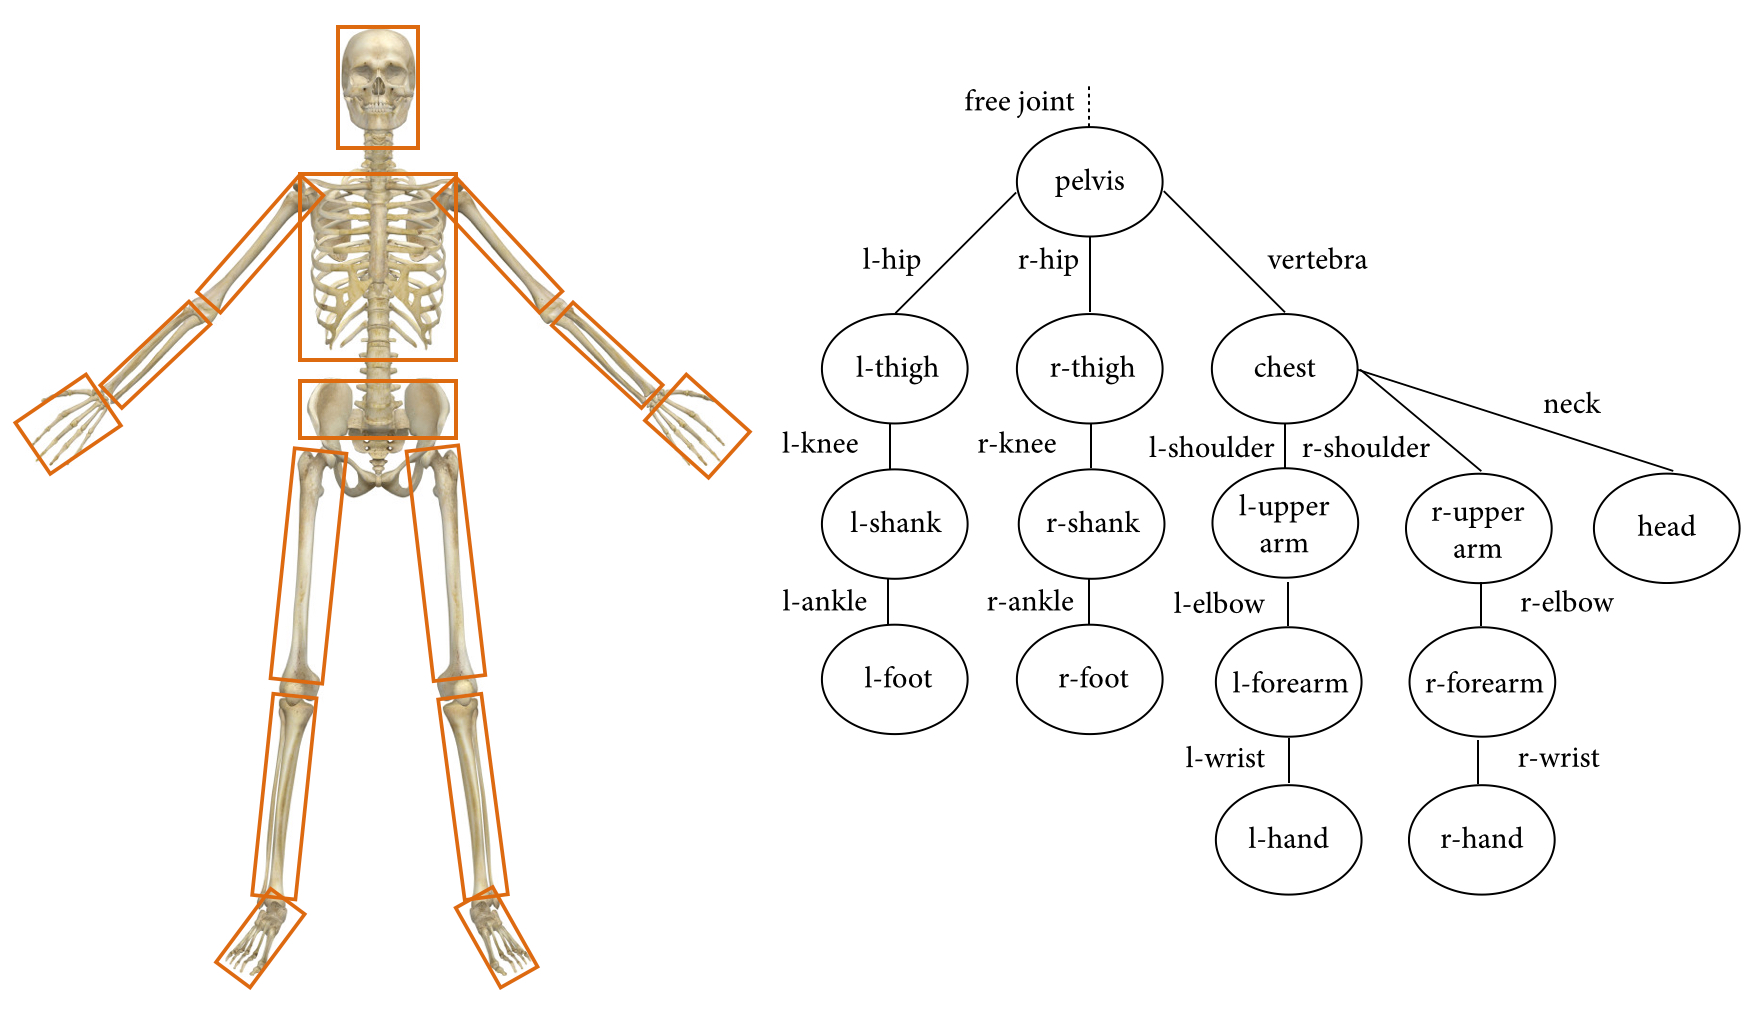
\includegraphics[width=6.0in]{skeletonTree.jpg}
\caption{Tasks for each research aim.}
\label{fig:skeleton}
\end{figure*}
 In DART, an articulated dynamics model is represented by a \textbf{Skeleton}. A Skeleton is a tree structure that consists of \textbf{BodyNode}s which are connected by \textbf{Joint}s. Every Joint has a child BodyNode, and every BodyNode has a parent Joint. Even the root BodyNode has a Joint that attaches it to the \textbf{World}. For example, the human skeleton can be organized into a tree structure (Figure \ref{fig:skeleton}) with nodes representing BodyNodes and edges representing Joints. Depending on the joint type (Section \ref{sec:jointTypes}), each joint has a specific number of degrees of freedom (DOFs). For example, the hip joint can be modeled by an \textbf{EulerJoint} with three DOFs, while a knee joint can be modeled by a \textbf{RevoluteJoint} with one DOF. In this model, we select the pelvis to be the root BodyNode, which connects to the World via a \textbf{FreeJoint} with six DOFs.

A kinematic chain is a sequence of transformations from one BodyNode to another in the Skeleton. Figure \ref{fig:parentChild}(a) illustrates the transformations between two intermediate BodyNodes denoted as Parent and Child. The coordinate frames of Parent, Child, and the joint between them are shown as the RGB arrows. Let $\vc{T}_{pj}$ be the transformation from the Parent frame to the joint frame and $\vc{T}_{cj}$ be the transformation from the Child frame to the joint frame. These two transformations are fixed and can be customized as part of the \textbf{Joint::Properties} of the joint. The transformation of the joint $\vc{T}(\vc{q})$ is a function of the DOFs, $\vc{q}$, associated with the joint. In the case of the hip joint, $\vc{q}$ is a 3x1 vector consisting of hip rotation angles in three dimensions. Thus, the transformation from the Parent frame to the Child frame is denoted by $\vc{T}_{pj}\vc{T}(\vc{q})\vc{T}_{cj}^T$.

\begin{figure*}
\centering
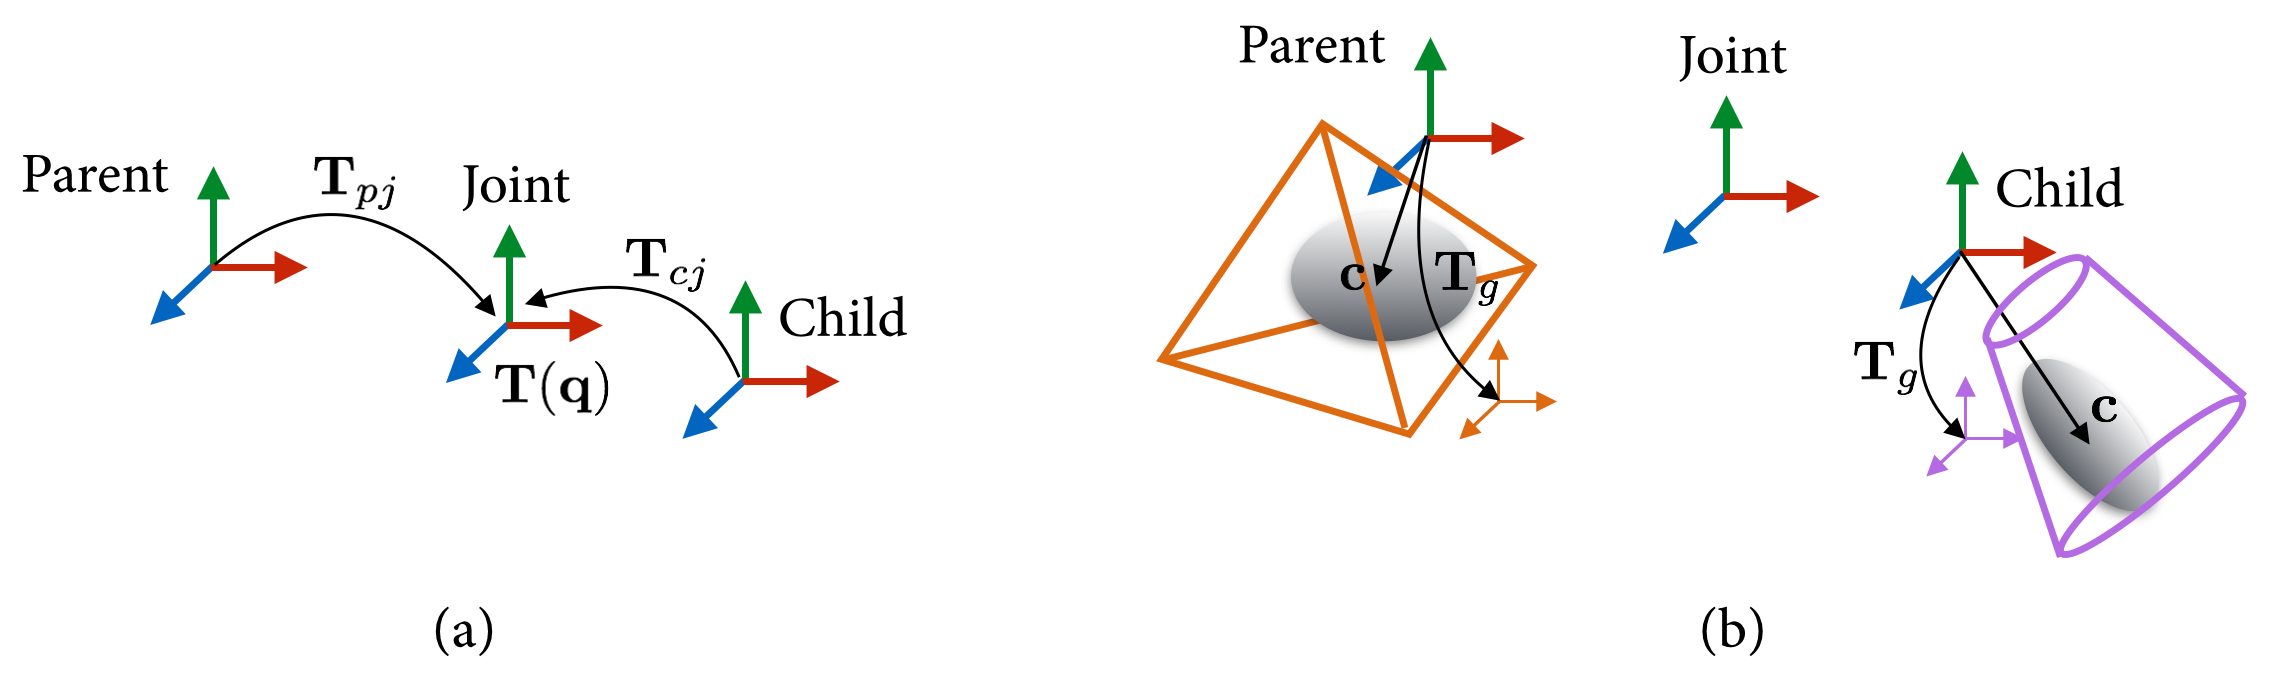
\includegraphics[width=6.0in]{parentChild.jpg}
\caption{Tasks for each research aim.}
\label{fig:parentChild}
\end{figure*}


\subsection{BodyNode Properties}
A BodyNode contains a set of customizable \textbf{BodyNode::Properties} to define its kinematic and dynamic behaviors.
\begin{itemize}[leftmargin=*] \itemsep1pt \parskip0pt \parsep0pt
  \item{\textbf{Inertial properties:}} The user can define the mass, the position of the center of mass in the BodyNode frame, and the moment of inertia around the center of mass in the BodyNode frame. The ellipsoids in Figure \ref{fig:parentChild}(b) illustrate the center of mass ($\vc{c}$) and the moment of inertia defined in the BodyNode frame.
  
\todo[MXG]{We should probably mention ShapeNode when discussing geometry}

  \item{\textbf{Geometry properties:}} The user can associate a set of \textbf{Shape}s with a BodyNode. Each shape has its own geometry information used by rendering and collision detection routines. DART supports a few primitive shapes, box, ellipsoid, cylinder, plane, line segment, in addition to arbitrary 3D polygons. Each shape can be defined in its own coordinate frame. The spatial relation between the Shape and its associated BodyNode is defined by a fixed transformation $\vc{T}_g$ (Figure \ref{fig:parentChild}(b)).
  \item{\textbf{Collision properties:}} The user can set the friction coefficient and the coefficient of restitution of a BodyNode, as well as the flag that determines whether the BodyNode is collidable.
\end{itemize}

\subsection{Joint types}
\label{sec:jointTypes}
DART supports 10 types of joints. Each joint type has a fixed number of DOFs and a specific configuration domain. Some joint types require the user to define their \textbf{UniqueProperties}. For example, the rotation axes of \textbf{RevoluteJoint}, \textbf{UniversalJoint} and \textbf{PlanarJoint} need to be specified when the joint is constructed. Likewise, the order of three axes (`xyz', `zyx', etc) in an \textbf{EulerJoint} needs to be predefined. These properties can be changed at any time, and the kinematics and dynamics calculations will automatically adjust to account for those changes. The only potential negative impact would be non-physical discontinuities if property changes are made during a simulation. Note that both \textbf{BallJoint} and \textbf{EulerJoint} are used to represent rotational motion in 3D space. However, a \textbf{BallJoint} is represented by an exponential map while an \textbf{EulerJoint} is represented by three consecutive 1D rotational matrices. All joint types provided by DART are listed in Table \ref{tab:jointTypes}.

\begin{table}[h]
\centering
\caption{Joint Types}
\begin{tabular}{|c|c|c|c|}
  \hline
  \textbf{Name} & \textbf{\#DOF} & \textbf{Configuration Domain}  & \textbf{Unique Properties}\\
  \hline
  BallJoint  &  3 & $SO(3)$  & \\
  \hline
  EulerJoint & 3  & $SO(2) \times SO(2) \times SO(2)$ & 3-axis order \\
  \hline
  FreeJoint  & 6 & $SE(3)$  &\\
  \hline
  PlanarJoint & 3  & $SE(2)$ & axis1 and axis2 \\
  \hline
  PrismaticJoint & 1  & $R$ & axis \\
  \hline
  RevoluteJoint & 1  & $SO(2)$ & axis \\
  \hline
  ScrewJoint & 1  & $SO(2)$ & axis and pitch \\
  \hline
  TranslationalJoint & 3  & $R^3$ &  \\
  \hline
  UniversalJoint & 2  & $SO(2) \times SO(2)$ & axis1 and axis2 \\
  \hline
  WeldJoint & 0  & $\emptyset$ &  \\
  \hline
\end{tabular}
\label{tab:jointTypes}
\end{table}

\subsection{Frame semantics}
Mathematical formulae are often expressed in terms of reference frames. This can make it difficult to directly program the formulae if your kinematic library is less expressive than the mathematical language. If a kinematic library only offers a frame's transformation with respect to its parent frame or the world frame, then you may need to repeatedly compute relative transformations between two arbitrary frames, which can easily introduce errors due to typos or confusion. Worse yet, the formulae for computing relative velocities and relative accelerations in non-inertial reference frames can be exceedingly complex and difficult to implement correctly. Take for example the equation to compute the relative linear acceleration of \textbf{Frame B} relative to \textbf{Frame A} in the coordinates of \textbf{Frame F}:

\begin{equation}
\label{eqn:rel_accel}
^{F}a_{BA} = ^{F}R_{O} ( ^{O}a_{B} - ^{O}a_{A} - ^{O}\dot{\omega}_{A} \times ^{O}p_{BA} - 2 ^{O}\omega_{BA} \times ^{O}v_{BA} - ^{O}\omega_A \times (^{O}\omega_{A} \times ^{O}p_{BA})
\end{equation}

Any small mistake, such as mixing up a plus with a minus or mixing up two of the variables, will produce potentially devastatingly incorrect results. Even the individual variables in the above expression each has a non-trivial formula to compute it, which must be implemented perfectly in order for any computations to come out correctly. These issues can pose considerable barriers to writing complex controller logic which is reliable enough to safely run on expensive robots.

KIDO addresses this issue by providing frame semantics. The forward kinematics of KIDO are handled by the underlying \textbf{Frame} class. The Frame class is a pure virtual class which provides the user with an interface to compute the kinematic values of a frame with respect to any other arbitrary frame. So instead of needing to implement equation \ref{eqn:rel_accel}, KIDO allows you to simply call the function:

\begin{lstlisting}
B->getLinearAcceleration(A,F);
\end{lstlisting}

Here are a few examples of what the Frame semantics API looks like:

\begin{lstlisting}
// Transformation Matrix
Eigen::Isometry3d Frame::getWorldTransform() const;
Eigen::Isometry3d Frame::getTransform(
    const Frame* withRespectTo = Frame::World()) const;

// Velocity
Eigen::Vector3d getLinearVelocity(
    const Frame* relativeTo = Frame::World(),
    const Frame* inCoordinatesOf = Frame::World()) const;
Eigen::Vector3d getAngularVelocity(
    const Frame* relativeTo = Frame::World(),
    const Frame* inCoordinatesOf = Frame::World()) const;
    
// Acceleration
Eigen::Vector3d getLinearAcceleration(
    const Frame* relativeTo = Frame::World(),
    const Frame* inCoordinatesOf = Frame::World()) const;
\end{lstlisting}

Note that an \textbf{Eigen::Isometry3d} is a specialized type of transformation matrix which exists in SE3.

Since \textbf{Frame} is a pure virtual interface class, we also need to have concrete implementations of it in order to perform forward kinematics. Most of the functions in \textbf{Frame} are actually implemented already; there are only five functions which derived classes need to implement:

\begin{lstlisting}
virtual const Eigen::Isometry3d& getRelativeTransform() const = 0;
virtual const Eigen::Vector6d& getRelativeSpatialVelocity() const = 0;
virtual const Eigen::Vector6d& getRelativeSpatialAcceleration() const = 0;
virtual const Eigen::Vector6d& getPrimaryRelativeAcceleration() const = 0;
virtual const Eigen::Vector6d& getPartialAcceleration() const = 0;
\end{lstlisting}

In the first three functions, the term \textit{Relative} means the quantity is relative to its parent frame. The first three functions are all that is needed to perform forward kinematics. The last two functions are used to reduce the number of computations when performing Featherstone's Articulated Body Algorithm for forward dynamics.

KIDO currently provides four concrete implementations of the \textbf{Frame} class:

\subsubsection{BodyNode Frame Implementation}

The \textbf{BodyNode} class is used to define the kinematic structure of a \textbf{Skeleton}. Because of this, it is very helpful for \textbf{BodyNode} to inherit the \textbf{Frame} class and be compatible with all of its forward kinematics and frame semantics features. The transformation, velocity, and acceleration of a \textbf{BodyNode} relative to its parent \textbf{Frame} is fully determined by its parent \textbf{Joint}. In the general case, it is not possible to explicitly move a \textbf{BodyNode} to an arbitrary transformation or give it an arbitrary velocity or acceleration. These physical quantities are all constrained by the parent \textbf{Joint} of the \textbf{BodyNode} as well as every \textbf{Joint} that it descends from. To achieve an arbitrary transformation for a \textbf{BodyNode}, KIDO offers an \textbf{InverseKinematics} module discussed later in this report \todo[MXG]{Link to InverseKinematics section}. KIDO does not currently offer an inverse differential kinematics module, but implementing one should be straightforward with the tools that KIDO does provide.

The BodyNode class and how to use it will be discussed in far greater detail throughout the rest of this report. In many ways, it is the cornerstone class of KIDO.

\subsubsection{SimpleFrame Implementation}

In some cases, it might be too cumbersome to be constrained by a \textbf{Joint} the way \textbf{BodyNode} is. If you want to have a reference \textbf{Frame} with a completely arbitrary transform, velocity, and acceleration, then being constrained by \textbf{Joint} can make things more difficult. Also, if you want your frame to represent a reference frame which is not a physical body, then the \textbf{BodyNode} class would be overkill.

For these reasons, we offer the \textbf{SimpleFrame} class. The \textbf{SimpleFrame} class is simply a Frame; it does not have any collision or inertial properties and therefore cannot be simulated. However, what \textbf{SimpleFrame} does offer is the ability to arbitrarily set its transformations, velocities, and accelerations. This can be done with the following functions:

\begin{lstlisting}
// Set transformation relative to parent Frame
void SimpleFrame::setRelativeTransform(const Eigen::Isometry3d& newRelTransform);

// Set transformation relative to any other Frame
void SimpleFrame::setTransform(
    const Eigen::Isometry3d& newTransform,
    const Frame* withRespectTo = Frame::World());
    
// Set the spatial velocity relative to the parent Frame, in the coordinates of this Frame
void SimpleFrame::setRelativeSpatialVelocity(
    const Eigen::Vector6d& newSpatialVelocity);
    
// Set the spatial velocity relative to the parent Frame, in the coordinates of any Frame
void SimpleFrame::setRelativeSpatialVelocity(
    const Eigen::Vector6d& newSpatialVelocity,
    const Frame* inCoordinatesOf);
    
// Set the spatial acceleration relative to the parent Frame, in the coordinates of this Frame
void SimpleFrame::setRelativeSpatialAcceleration(
    const Eigen::Vector6d& newSpatialAcceleration);

// Set the spatial acceleration relative to the parent Frame, in the coordinates of any Frame
void SimpleFrame::setRelativeSpatialAcceleration(
    const Eigen::Vector6d& newSpatialAcceleration,
    const Frame* inCoordinatesOf);
\end{lstlisting}

It is important to note that, by default, spatial quantities like spatial velocity and spatial acceleration should be given in the coordinates of the frame that they belong to (\textbf{not} in the coordinates of the parent frame). But KIDO does provide convenience functions that allow you to represent the spatial quantities in whichever coordinates you would like to. However, they still must represent the quantities \textbf{relative to} the parent, even if they're expressed in the coordinates of a different frame (i.e. the values are rotated).

For those who are not familiar or not comfortable with spatial quantities, KIDO also offers an API for classic 3D vectors, like those used in the traditional Newton-Euler equations of motion:

\begin{lstlisting}
void SimpleFrame::setClassicDerivatives(
    const Eigen::Vector3d& linearVelocity      = Eigen::Vector3d::Zero(),
    const Eigen::Vector3d& angularVelocity     = Eigen::Vector3d::Zero(),
    const Eigen::Vector3d& linearAcceleration  = Eigen::Vector3d::Zero(),
    const Eigen::Vector3d& angularAcceleration = Eigen::Vector3d::Zero());
\end{lstlisting}

Even though KIDO provides an API that supports both spatial and classic vectors, under the hood it only utilizes spatial vectors, because spatial vectors require fewer operations for forward differential kinematics. This also means that only spatial vectors get stored under the hood, and therefore if a user wants to set the velocity and/or acceleration using classic vectors, then all classic vectors must be provided simultaneously, or else the final result would depend on the order in which the classic vectors get set, which would be confusing and undesirable behavior.

\subsubsection{FixedFrame Implementation}

The \textbf{BodyNode} frame implementation is constrained by Joints while the \textbf{SimpleFrame} frame implementation is completely unconstrained. The \textbf{FixedFrame} implementation allows the user complete freedom in setting the initial relative transform, but after that it may not move. Its relative velocity and relative acceleration vectors are always exactly zero. \textbf{FixedFrame} instances do not even offer a way to change the relative transform after construction.

However, it is still possible for a class to inherit the \textbf{FixedFrame} class, and the inheriting class does have the authority to alter the relative transform. For example, the \textbf{EndEffector} class is a derivative of \textbf{FixedFrame} and allows the user to change the relative transform freely. But no matter how the relative transform gets changed, the relative velocity and relative acceleration will always be reported as zero, so altering a relative transform during a simulation could result in non-physical discontinuities.

\subsubsection{WorldFrame Implementation}

The \textbf{WorldFrame} is a very special case of the \textbf{Frame} class. It always returns identity for its relative transformation as well as its world transformation. Its velocities and accelerations are always zero. It is a singleton class which only gets created once per program, and every kinematic chain descends from it. To access the \textbf{WorldFrame}, simply call the function \textbf{Frame::World()}.

Conventional wisdom and good software engineering practices dictate that singletons should be avoided almost always. In the case of the \textbf{WorldFrame}, it is designed to be a read-only object whose values are never changed. Therefore it is not at risk of issues related to race conditions or unexpected interdependencies within the code.

\subsection{Kinematic state of the system}
DART provides a variety of ways to query the position and the velocity of the system in generalized, Cartesian, and spatial coordinates. 

\begin{lstlisting}
// Generalized coordinates
Eigen::VectorXd MetaSkeleton::getPositions() const;
Eigen::VectorXd MetaSkeleton::getVelocities() const;

// Cartesian coordinates
Eigen::Isometry3d Frame::getTransform(const Frame* _withRespectTo = Frame::World(), const Frame* _inCoordinatesOf = Frame::World()) const;
Eigen::Vector3d Frame::getLinearVelocity(const Eigen::Vector3d& _offset, const Frame* _relativeTo = Frame::World(), const Frame* _inCoordinatesOf = Frame::World()) const;
Eigen::Vector3d Frame::getAngularVelocity(const Frame* _relativeTo = Frame::World(), const Frame* _inCoordinatesOf = Frame::World()) const;
Eigen::Vector3d Skeleton::getCOM(const Frame* _withRespectTo = Frame::World()) const override;
Eigen::Vector3d Skeleton::getCOMLinearVelocity(const Frame* _relativeTo = Frame::World(), const Frame* _inCoordinatesOf = Frame::World()) const override;
Eigen::Vector3d BodyNode::getCOM(const Frame* _withRespectTo = Frame::World()) const;
Eigen::Vector3d BodyNode::getCOMLinearVelocity(const Frame* _relativeTo = Frame::World(), const Frame* _inCoordinatesOf = Frame::World()) const;

// Spatial coordinates
Eigen::Vector6d Frame::getSpatialVelocity(const Eigen::Vector3d& _offset, const Frame* _relativeTo, const Frame* _inCoordinatesOf) const;
\end{lstlisting}

For  example, if one wishes to know the transformation of the left
hand from the left upper arm expressed in the coordinate frame of the
pelvis, it can be achieved by 

\begin{lstlisting}
// Assume l-hand, l-upper-arm, and pelvis are pointers of BodyNode
 Isometry3d T = l-hand->getTransform(l-upper-arm, pelvis);
\end{lstlisting}

The velocity of any point in any BodyNode frame relative to any other
frame can be queried. For example, the relative linear velocity of a
local point, \emph{offset}, in the \emph{l-hand} frame from the origin of the \emph{l-upper-arm} frame expressed in the \emph{pelvis} frame can be accessed by

\begin{lstlisting}
 Vector3d v = l-hand->getLinearVelocity(offset, l-upper-arm, pelvis);
\end{lstlisting}


% \paragraph{Generalized coordinates.} The configuration of a skeleton can be accessed via the functions that return the generalized positions of a system.

% \begin{lstlisting}[caption=MetaSkeleton.h]
% // Get the positions for all generalized coordinates
% Eigen::VectorXd getPositions() const;

% // Get the positions for a subset of the generalized coordinates
% Eigen::VectorXd getPositions(const std::vector<size_t>& _indices) const;

% // Get the position of a single generalized coordinate
% double getPosition(size_t _index) const;

% // Get the velocities for all generalized coordinates
% Eigen::VectorXd getVelocities() const;

% // Get the velocities for a subset of the generalized coordinates
% Eigen::VectorXd getVelocities(const std::vector<size_t>& _indices) const;

% // Get the velocity of a single generalized coordinate
% double getVelocity(size_t _index) const;
% \end{lstlisting}

% \paragraph{Cartesian coordinates.}DART provides flexible API to query the transformation of a BodyNode relative expressed in any coordinate frame, with respect to any coordinate frame. 

% \begin{lstlisting}[caption=Frame.h]
% // Example: The transformation of the left hand from the left upper arm expressed in the coordinate frame of the pelvis can be accessed by 
% // Isometry3d T = l-hand->getTransform(l-upper-arm, pelvis);
% // , where l-hand, l-upper-arm, and pelvis are pointers of BodyNode.
 
% Eigen::Isometry3d getTransform(const Frame* _withRespectTo = Frame::World(), const Frame* _inCoordinatesOf = Frame::World()) const;
% \end{lstlisting}

% In the absence of the second and the third arguments, this function will return the transformation from the World to the BodyNode expressed in the World frame.

% In terms of Cartesian velocity, the linear velocity of any point in any BodyNode frame relative to any other frame can be queried. This linear velocity can be expressed in any coordinate frame. We can also query the angular velocity of a BodyNode relative to any other frame expressed in any frame.

% \begin{lstlisting}[caption=Frame.h]
% // Example: The relative linear velocity of a local point ''Vector3d offset(0.1, 0, 0)'' in the l-hand frame from the origin of the l-upper-arm frame expressed in the pelvis frame can be accessed by
% // Vector3d v = l-hand->getLinearVelocity(offset, l-upper-arm, pelvis);

% Eigen::Vector3d getLinearVelocity(const Eigen::Vector3d& _offset, const Frame* _relativeTo = Frame::World(), const Frame* _inCoordinatesOf = Frame::World()) const;

% Eigen::Vector3d getAngularVelocity(const Frame* _relativeTo = Frame::World(), const Frame* _inCoordinatesOf = Frame::World()) const;
% \end{lstlisting}

% DART also provides convenient API to access the state of the center of mass for a Skeleton.

% \begin{lstlisting}[caption=Skeleton.h]
% Eigen::Vector3d getCOM(const Frame* _withRespectTo = Frame::World()) const override;

% Eigen::Vector3d getCOMLinearVelocity(const Frame* _relativeTo = Frame::World(), const Frame* _inCoordinatesOf = Frame::World()) const override;
% \end{lstlisting}

% The same API is also provided for accessing the state of the center of mass for a BodyNode.

% \begin{lstlisting}[caption=BodyNode.h]
% Eigen::Vector3d getCOM(const Frame* _withRespectTo = Frame::World()) const;

% Eigen::Vector3d getCOMLinearVelocity(const Frame* _relativeTo = Frame::World(), const Frame* _inCoordinatesOf = Frame::World()) const;
% \end{lstlisting}

% \paragraph{Spatial coordinates.}

\subsection{Jacobian matrices}
Calculating Jacobian matrix is a common theme in forward simulation, inverse kinematics, and many other robotics or graphics applications. DART computes Jacobian matrices and its derivatives efficiently and provides API to access the results in various forms. 

\paragraph{Skeleton.} The full Jacobian matrix with respect to all DOFs in the system can be accessed via the member functions of Skeleton.

\begin{lstlisting}[caption=Skeleton.h]
math::LinearJacobian getLinearJacobian(const BodyNode* _bodyNode, const Eigen::Vector3d& _localOffset, const Frame* _inCoordinatesOf = Frame::World()) const override;

math::AngularJacobian getAngularJacobian(const BodyNode* _bodyNode, const Frame* _inCoordinatesOf = Frame::World()) const override;
\end{lstlisting}

The first function returns $J_v$ that maps the generalized velocity of
the system to the velocity of the point attached to \emph{bodyNode}
with an offset, \emph{localOffset}, from the origin of
\emph{bodyNode}, $\vc{v} = J_v \dot{\vc{q}}$. The second function
returns $J_{\omega}$ that maps the generalized velocity to the angular
velocity of \emph{bodyNode}, $\omega = J_{\omega}\dot{\vc{q}}$. The
last optional parameter, \emph{inCoordinatesOf}, determines in which
coordinate frame the Jacobian matrix is expressed. The full Jacobian
matrix that combines both $J_v$ and $J_{\omega}$ can be obtained by
the following function.

\begin{lstlisting}[caption=Skeleton.h]
math::Jacobian getJacobian(const BodyNode* bodyNode, const Eigen::Vector3d& localOffset, const Frame* inCoordinatesOf) const override;
\end{lstlisting}


% $R^T\frac{\partial T\vc{p}}{\partial \vc{q}} \in \vc{R}^{3\times n}$,
% where $R$ is the rotation part of the transformation from the World
% frame to the frame of \emph{inCoordinatesOf}, $T$ is the
% transformation from the World frame to the frame of \emph{BodyNode},
% $\vc{p}$ is a local coordinate indicated by \emph{localOffset} in the
% frame of \emph{bodyNode}, and $\vc{q}$ is the vector of DOFs of the
% system which has the size $n$. The second function returns 


% The submatrix containing the top three
% rows is the linear Jacobian matrix of the point attached to
% \emph{bodyNode} with an offset, \emph{localOffset}, from the origin of
% \emph{bodyNode}, while the submatrix containing the bottom three rows
% is the angular Jacobain matrix of the \emph{bodyNode} frame. The
% Jacobain matrix can be expressed in any coordinate frame specified by
% \emph{inCoordinatesOf}. If only linear or angular Jacobian matrix is
% needed, the following two functions can be used.


\paragraph{BodyNode.} More compact Jacobian matrices can be acquired
via the member functions of a BodyNode. Unlike the Jacobain matrices
for the entire Skeleton, these Jacobian matrices have $m$ columns, the number of DOFs on the kinematic chain from the root node to the BodyNode of interest.


\begin{lstlisting}[caption=BodyNode.h]
math::LinearJacobian getLinearJacobian(const Eigen::Vector3d& _offset, const Frame* _inCoordinatesOf = Frame::World()) const;

math::AngularJacobian getAngularJacobian(const Frame* _inCoordinatesOf = Frame::World()) const;

math::Jacobian getJacobian(const Eigen::Vector3d& _offset, const Frame* _inCoordinatesOf) const;
\end{lstlisting}

\paragraph{Joint.} Similar Jacobian functions are also available for
the Joint class. The number of columns of the Jacobian depends on the
number of DOFs of the joint. For example, a BallJoint returns a $6
\times 3$ Jacobian while a RevoluteJoint returns a $6 \times 1$ Jacobian.

\begin{lstlisting}[caption=Joint.h]
virtual math::Jacobian getLocalJacobian(const Eigen::VectorXd&
_positions) const = 0;
\end{lstlisting}



% Joint:
% /// Get generalized Jacobian from parent body node to child body node
%   /// w.r.t. local generalized coordinate
%   virtual const math::Jacobian getLocalJacobian() const = 0;

%   /// Get generalized Jacobian from parent body node to child body node
%   /// w.r.t. local generalized coordinate
%   virtual math::Jacobian getLocalJacobian(
%       const Eigen::VectorXd& _positions) const = 0;

%   /// Get time derivative of generalized Jacobian from parent body node
%   /// to child body node w.r.t. local generalized coordinate
%   virtual const math::Jacobian getLocalJacobianTimeDeriv() const = 0;

\subsection{Skeleton modeling}
Building a complex skeleton from scratch can be very
difficult and tedious. Often time, the developer may prefer to modify an
existing skeleton described by a URDF or SDF file. DART provides many
functions to facilitate skeleton editing summarized in the following
table.

\begin{table}[h]
\centering
\caption{Functions for Skeleton Modeling}
\begin{tabular}{|L{3.3in}|L{2.7in}|}
  \hline
  \textbf{Function Example} & \textbf{Description} \\
  \hline
  bd1-$>$\textbf{remove}() & Remove BodyNode bd1 and its subtree from their Skeleton.  \\
  \hline
   bd1-$>$\textbf{moveTo}(bd2) & Move BodyNode bd1 and its subtree under BodyNode bd2.  \\
  \hline
 auto newSkel = bd1-$>$\textbf{split}("new skeleton") & Remove BodyNode bd1 and its subtree from their current Skeleton and move them into a newly created Skeleton named "new skeleton".  \\
  \hline
 bd1-$>$\textbf{changeParentJointType}$<$BallJoint$>$() & Change the joint type of BodyNode bd1's parent joint to BallJoint.  \\
  \hline
bd1-$>$\textbf{copyTo}(bd2) & Create a clone of BodyNode bd1 and its subtree
                   and attach the clone to an existing BodyNode bd2. \\
  \hline
 auto newSkel = bd1-$>$\textbf{copyAs}("new skeleton") & Create a
                                                         clone of
                                                         BodyNode bd1
                                                         and its
                                                         subtree as a new skeleton named "new skeleton".  \\
  \hline
\end{tabular}
\label{tab:skeletonEdit}
\end{table}

Some functions have optional parameters for more advanced modeling
operations. For example, \textbf{moveTo} is templated by \textbf{JoinType} and
can take in \textbf{Joint::Properties} as an argument, such as:
bd1->moveTo<EulerJoint>(bd2, properties).

\subsection{Inverse kinematics}
\red{Grey}

\section{Dynamic Features}
Physics simulation is the core mission of DART. The earlier versions of DART
adopted the physics engine, RTQL8 \cite{}, which features forward
simulation based on Lagrangian dynamics
and generalized coordinates. Later, we reimplemented the Featherstone
algorithms using Lie group representation to largely improve the
computation efficiency. The constraint solver, which handles contact,
joint limits, and other Cartesian constraints, has also been optimized
in the later versions of DART. 

\subsection{Lagrangian dynamics and generalized coordinates}
DART is distinguished by its accuracy and stability due to its use of
generalized coordinates to represent articulated rigid body systems,
Featherstone’s algorithm to compute the dynamics of
motion, and Lie group for compact representation and derivation of
dynamic equations.

Articulated human motions can be described by a set of dynamic
equations of motion of multibody systems. Since the direct application
of Newton’s second law becomes difficult when a complex articulated
rigid body system is considered, we use Lagrange’s equations derived
from D'Alembert’s principle to describe the dynamics of motion: 
\begin{equation}
M(\vc{q})\ddot{\vc{q}} + C(\vc{q}, \dot{\vc{q}}) = \vc{Q},
\end{equation}
where $\vc{q}$ is the generalized coordinates that indicate the 
configuration of the skeleton. $M(\vc{q})$ is the mass matrix,
$C(\vc{q},\dot{\vc{q}})$ is the Coriolis and centrifugal term of the
equation of motion, and $\vc{Q}$ is the vector of generalized forces
for all the degrees of freedom in the system.

Once we know how to compute the mass matrix, Coriolis and centrifugal
terms, and generalized forces, we can compute the acceleration in
generalized coordinates, $\ddot{\vc{q}}$ for forward dynamics. Conversely, if we
are given $\ddot{\vc{q}}$ from a motion sequence, we can use these equations of
motion to derive generalized forces for inverse dynamics. However,
directly evaluating the mass matrix and Coriolis term is 
computationally expensive, especially for applications that require
real-time simulation. DART implements Featherstone's articulated rigid
body algorithms to compute forward and inverse dynamics. In addition,
DART uses Lie group representation to further improve efficiency.

\paragraph{Featherstone's algorithms.} In particular, we implement the
recursive Newton-Euler algoritm (RNEA) for inverse dynamics and the
articulated-body algorithm (ABA) for forward dynamics. These two
algorithms are known for their $O(n)$ time with $n$ being the number of
body nodes in the skeleton. 

\paragraph{Lie group representation}
\red{JS} (Describe the high-level ideas of Lie group representation and its advantages).

\subsection{Soft body simulation}
DART is able to simulate soft bodies dynamically coupling with rigid
bodies. For example, one can simulate a robotic gripper with deformable
surface or a humanoid with rubber soles on the feet. The soft body
simulation in DART is based on spring-mass systems described in
generalized coordinates. We use a unified representation for both
rigid and soft bodies so that two-way dynamic coupling can be handled
by the same set of equations of motion (Figure \ref{fig:softbody}. 

\begin{figure*}
\centering
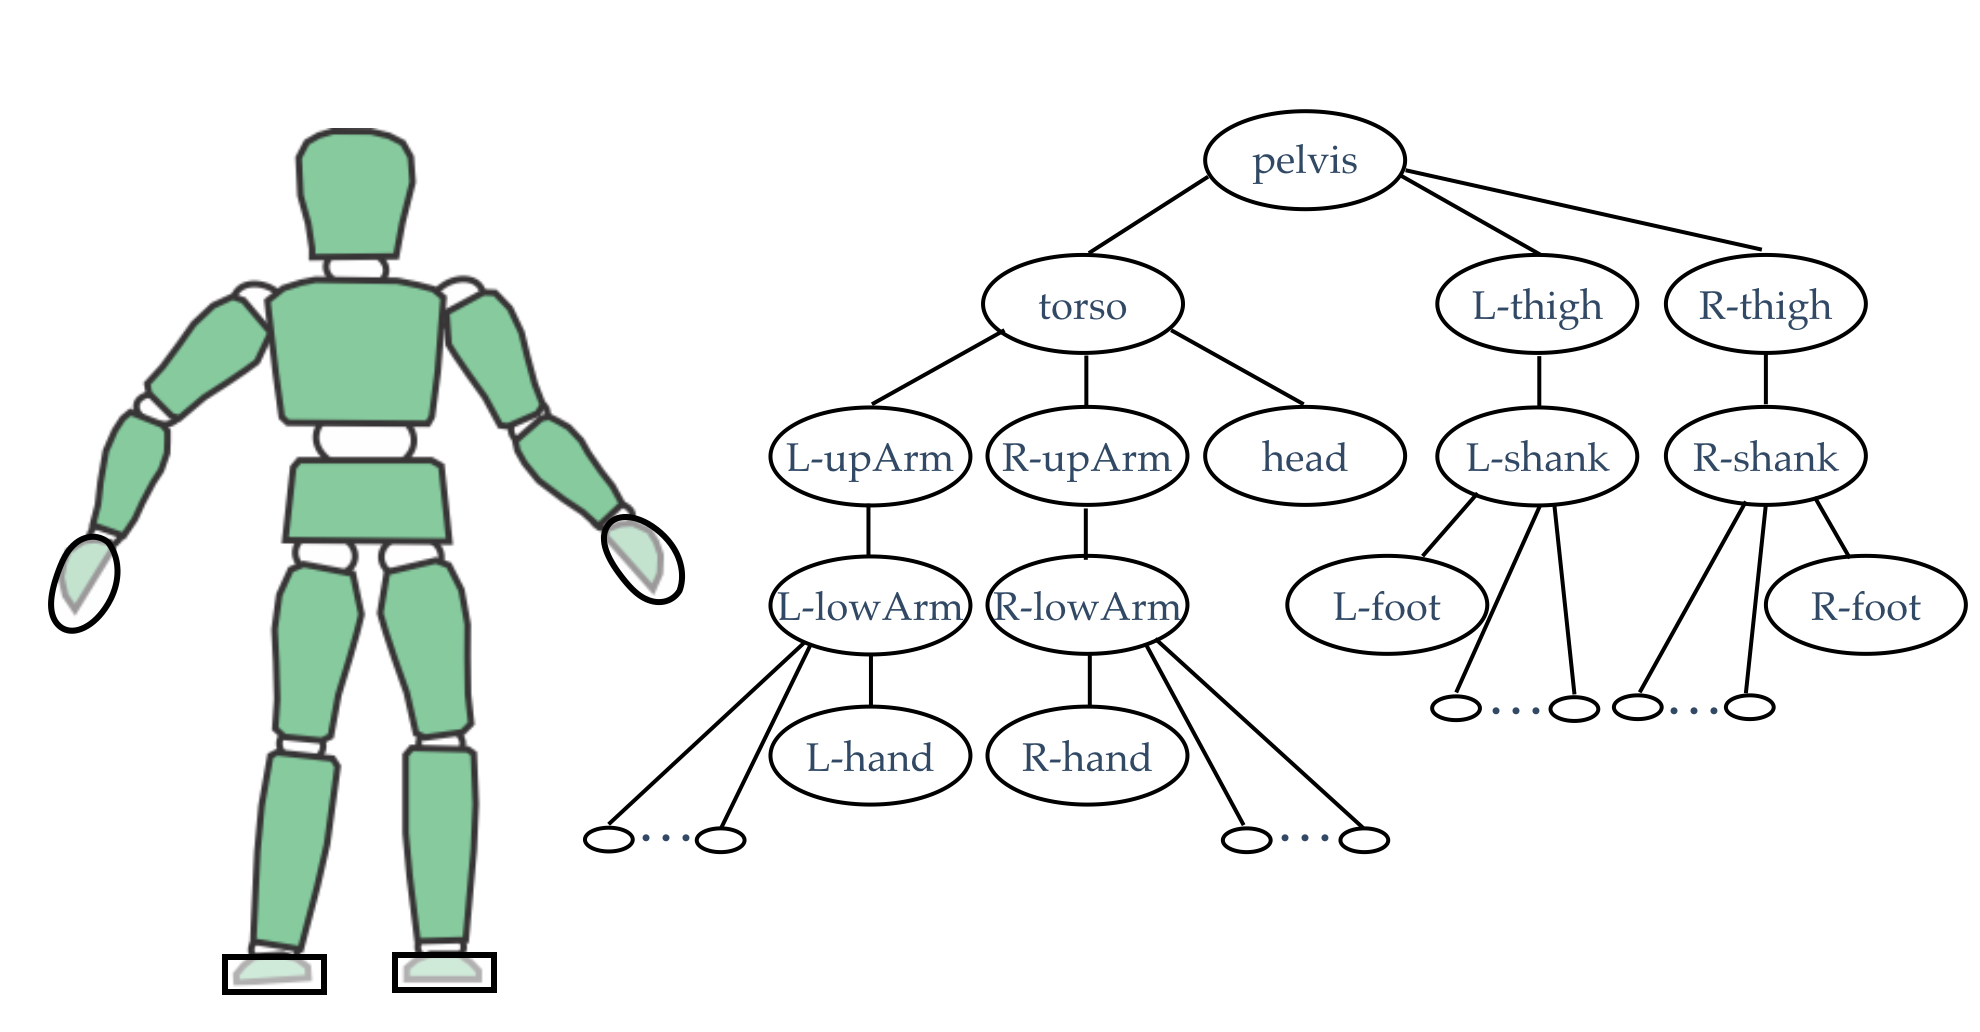
\includegraphics[width=6.0in]{fig/soft-body.jpg}
\caption{The hands and the feet of the humanoid are composed of a
  rigid body with a layer of deformable surface. Both rigid and soft
  bodies are represented in generalized coordinates.}
\label{fig:softbody}
\end{figure*}

Each SoftBodyNode consists of a set of point masses representing the
surface of the deformable part of the body. Each point mass is
attached to the frame of BodyNode as a child link with three translational
degrees of freedom. This compact representation allows us to soften or
harden any part of deformable body at any time, by simply adding or
removing the translational degrees of freedom of involved point
masses, without switching dynamic regimes or introducing any
instability. Based on this flexible representation, we develop an
efficient system where only the site of collision needs to be
simulated as deformable body while the rest of the character remains
rigid.

To make a BodyNode soft, one can simply add a
$<$soft\_shape$>$ element in the $<$body$>$ element in the SKEL file. For
example, if we want to make the left foot of the skeleton
``humanoid'' soft, we will modify the SKEL file as follows:

\begin{lstlisting}[caption=Joint.h]
 <skeleton name="humanoid">
 ...
   <body name="Left foot">
     <gravity>1</gravity>
     <transformation>0 -0.10 0 0 0 0</transformation>
     <inertia>
       <mass>0.5</mass>
       <offset>0 0 0</offset>
     </inertia>
     <soft_shape>
       <total_mass>0.5</total_mass>
       <geometry>
         <box>
           <size>0.5 0.25 0.5</size>
           <frags>3 3 3</frags>
         </box>
       </geometry>
       <kv>500.0</kv>
       <ke>0.0</ke>
       <damp>5.0</damp>
     </soft_shape>
   </body>
...
\end{lstlisting}

The material of the soft body is crucial to the behavior of the soft
body. DART uses four parameters to describe the characteristics of the
soft body:

\begin{enumerate}
\item{Number of point masses ($n$):} The resolution of the soft body surface. 
\item{Shape deformation coefficient ($K_e$):} This parameter
  affects the deformation of the soft body in its material space. 
\item{Surface displacement coefficient ($K_v$)}: This parameter
  affects the displacement of the soft body in the frame of the
  BodyNode. The displacement can be caused by the deformation of the
  shape and the rigid transformation relative to the BodyNode frame.
\item{Damping coefficient ($K_d$):} The damping coefficient of the spring.
\end{enumerate}

\subsection{Joint dynamics}
By default, a joint is completely passive, but DART also provides a
few parameters for the user to model a joint as an angular damped
spring with tunable rest pose, stiffness coefficient, and damping
coefficient.

\begin{lstlisting}[caption=Joint.h]
virtual void setRestPosition(size_t _index, double _q0);
virtual void setSpringStiffness(size_t _index, double _k);
virtual void setDampingCoefficient(size_t _index, double _coeff);
\end{lstlisting}

It is important to note that DART simulates joint dynamics using
implicit integration method which uses the future state to evaluate
the spring and damper forces. The implicit formulation results in
solving a linear system, which is more computational costly, but it
makes the system more stable and allows for larger time step in
simulation.

\subsection{Actuators}
\red{Karen}

\subsection{Constraints}
\red{JS}

\subsection{Accuracy and Performance}
\red{JS}

\section{Other Features}
\subsection{Collision detectors}
\red{JS}
\subsection{Integration methods}
\red{Karen}
\subsection{Lazy evaluation and automatic updating}
\label{sec:lazy}
Most kinematics libraries have a strict workflow that must be followed in order to produce correct results in a timely manner. Typically this workflow requires that all joint positions must be set and then all transforms must be computed before the transformation of a specific frame may be queried. This is a wasteful and inefficient approach for many applications.

For example, a dexterous robot manipulator may have seven links from the base to the end effector, but then it may have three fingers which each have three links. While iteratively performing inverse kinematics, it will be necessary to repeatedly compute the seven matrix transformations that go from the base to the end effector, but the transforms of the nine finger links are unnecessary. A naive approach to updating kinematics will compute all 16 transforms, even though only 7 are necessary. This means that over 56\% of the computational effort of the forward kinematics is wasted. When iteratively solving an inverse kinematics problem, the bulk of time is spent computing forward kinematics. This means that intelligently updating the forward kinematics could yield a nearly 50\% reduction in computation time for this example. Similar (and more extreme) examples could be imagined for robots with multiple limbs.

Strict workflow requirements can also lead to bugs in code. If a human programmer is not familiar with the correct workflow, does not fully understand the necessary order of operations, or simply makes a programming error, then there may be bugs in a complex controller which would produce incorrect results. Incorrect results on a dexterous manipulator could cause a task to fail and damage the robot. Incorrect results on a high-powered robot could severely damage the robot and even endanger human lives.

\subsubsection{Design}

KIDO resolves those concerns using lazy evaluation and automatic updating. Most kinematic and dynamic quantities in KIDO are automatically updated and lazily evaluated (see section \ref{sec:lazy_exception} for the exceptions). \textit{Automatic updating} means that you never need to explicitly call any kind of ``update'' function in order to get the correct output based on your most recent input. \textit{Lazy evaluation} means that expensive computations are held off until they are absolutely required by the user. Combined, these two add a decisive level of code safety to applications that use KIDO, and they cut out a considerable degree of potential waste, both while making the library easier to use. This is accomplished with the following setup:

\begin{itemize}
  \item Mutator and accessor methods (a.k.a. setters and getters) intercept all interactions with the internal states and properties of kinematic objects.
  \item Dirty flags are used to keep track of which quantities are out of date, and the dirtiness gets propagated to all dependencies.
  \item Accessor methods will check any relevant dirty flags and perform computations as necessary.
  \item Mutator methods will trigger dirty flags.
\end{itemize}

A visual example of this scheme applied to forward kinematics can be seen in figure \ref{fig:lazy}. Note that the propagation of dirty flags throughout the kinematic structure will short-circuit any time a kinematic object already knows that it is dirty. This prevents the bookkeeping from having $O(N^2)$ complexity when all $N$ joints in the kinematic structure undergo changes.

To facilitate this lazy evaluation, KIDO abides by logical const-correctness (rather than physical const-correctness). The values that are lazily evaluated are stored as mutable members of their class, allowing the \texttt{getX()} functions to be const member functions. However, because of this mutability, the const-qualifier on member functions does \textbf{not} guarantee thread-safety. Currently, the only guaranteed way to ensure thread-safety with KIDO is to spawn identical copies of the kinematic structures for each thread. This is done easily with the various \texttt{clone()} functions throughout KIDO. To spawn an identical copy of a single Skeleton, simply call \texttt{Skeleton::clone()} on it. To spawn an identical copy of a whole environment, you can use the \texttt{simulation::World::clone()} function.

\begin{figure}
  \centering
  \subfigure[][\label{fig:lazy_1}Everything is cached]{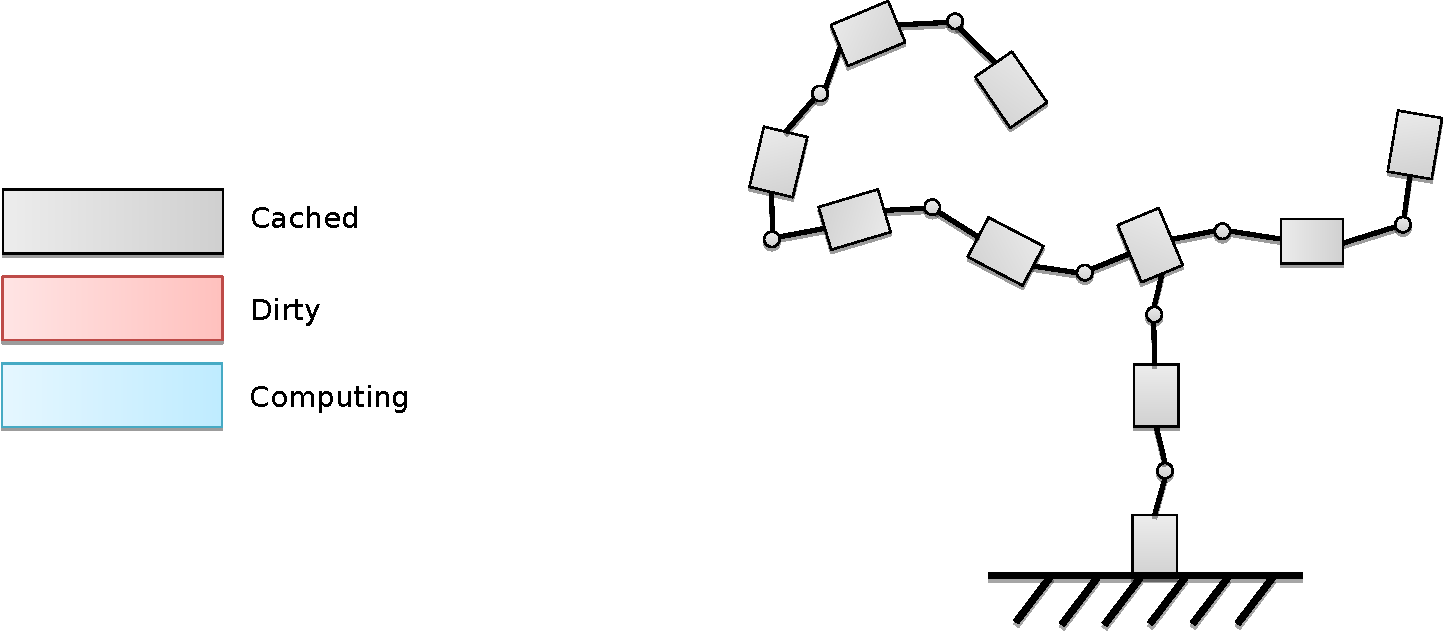
\includegraphics[width=0.98\textwidth]{fig/lazy_1.pdf}}
  
  \subfigure[][\label{fig:lazy_2}Some joint values have changed]{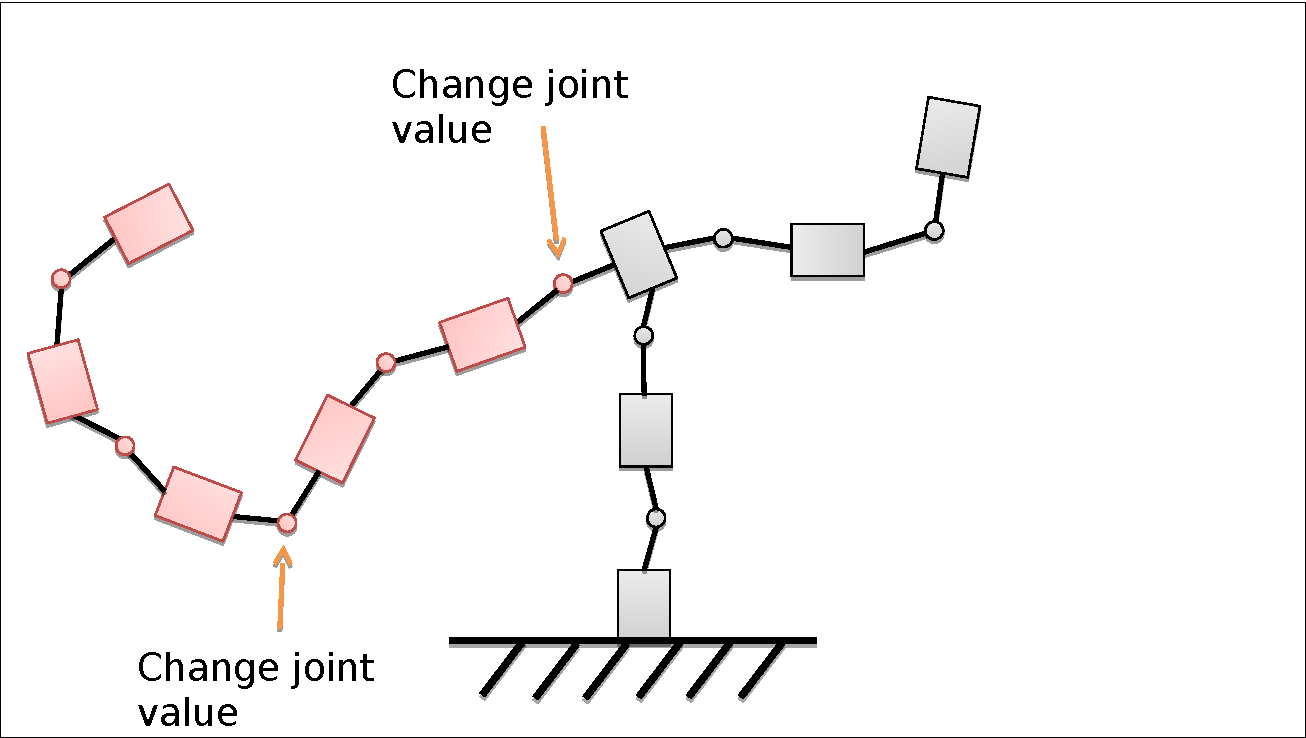
\includegraphics[width=0.44\textwidth]{fig/lazy_2.pdf}}
  \subfigure[][\label{fig:lazy_3}A dirty transform is queried]{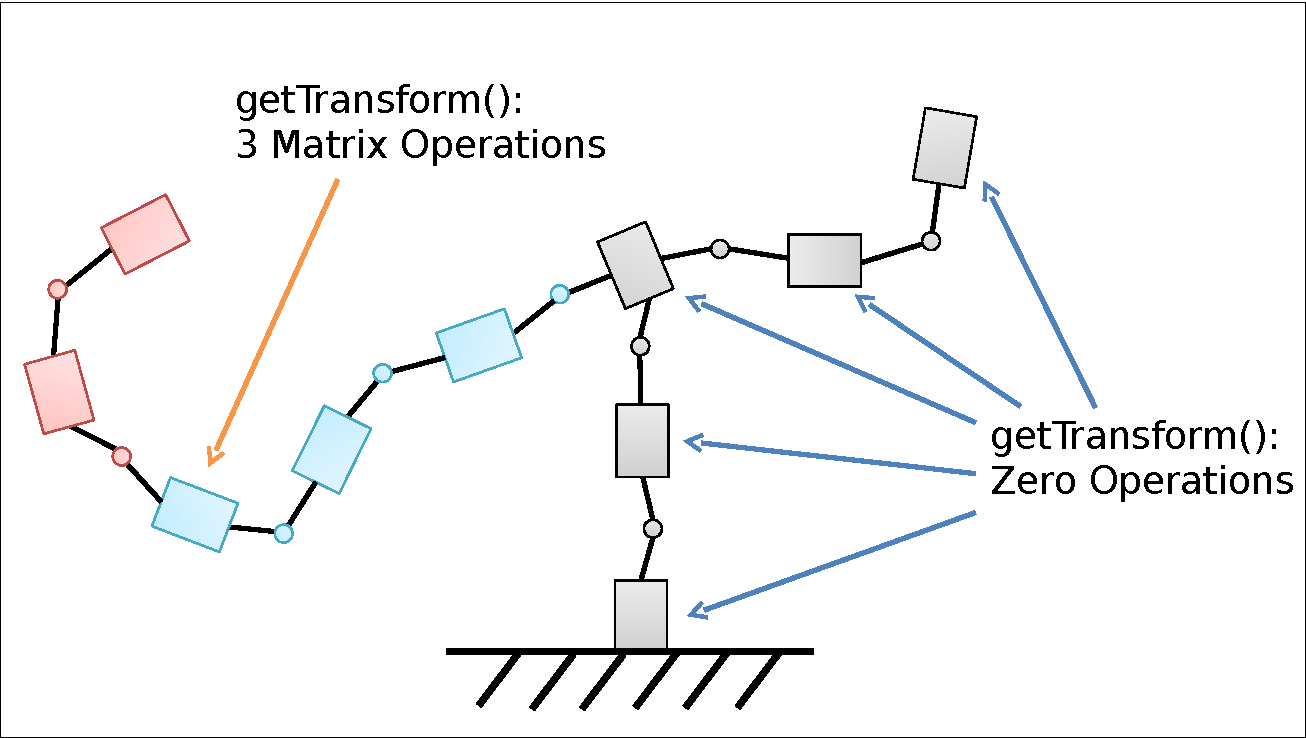
\includegraphics[width=0.44\textwidth]{fig/lazy_3.pdf}}
  
  \subfigure[][\label{fig:lazy_4}Cached transforms can be used freely]{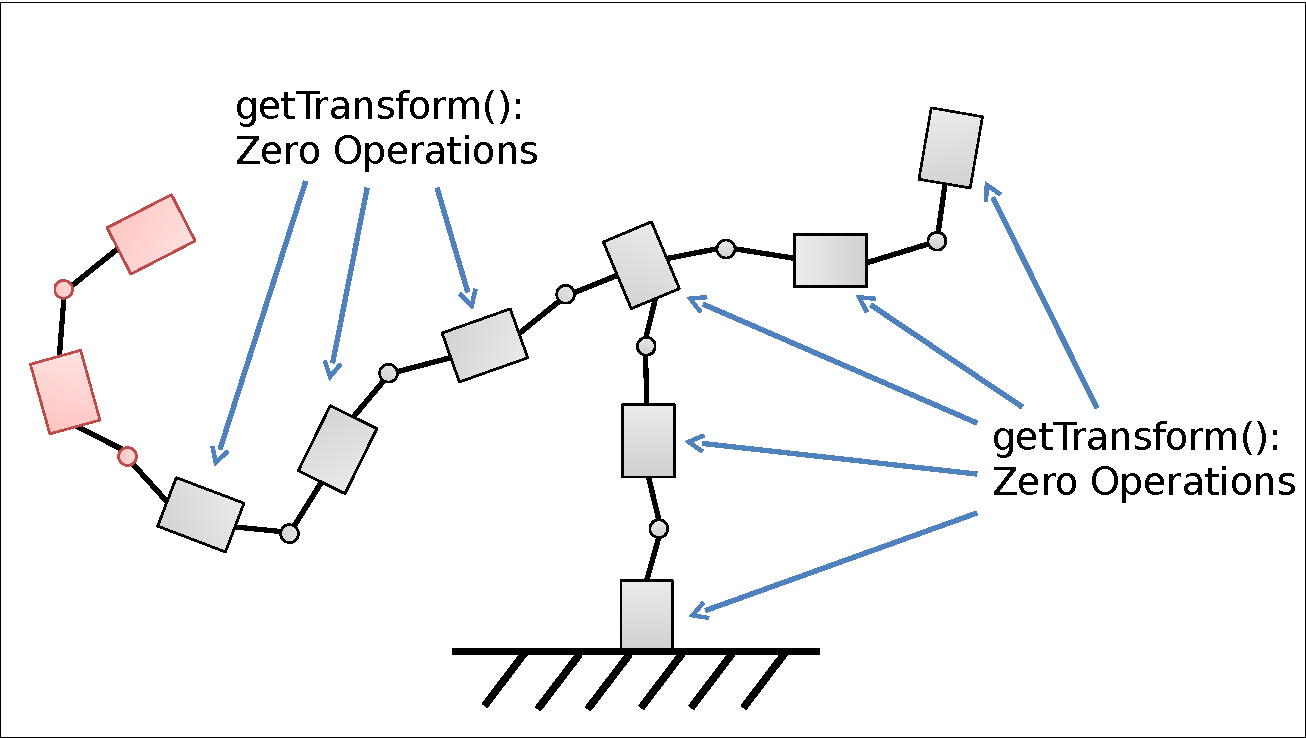
\includegraphics[width=0.44\textwidth]{fig/lazy_4.pdf}}
  \subfigure[][\label{fig:lazy_5}Another dirty transform is queried]{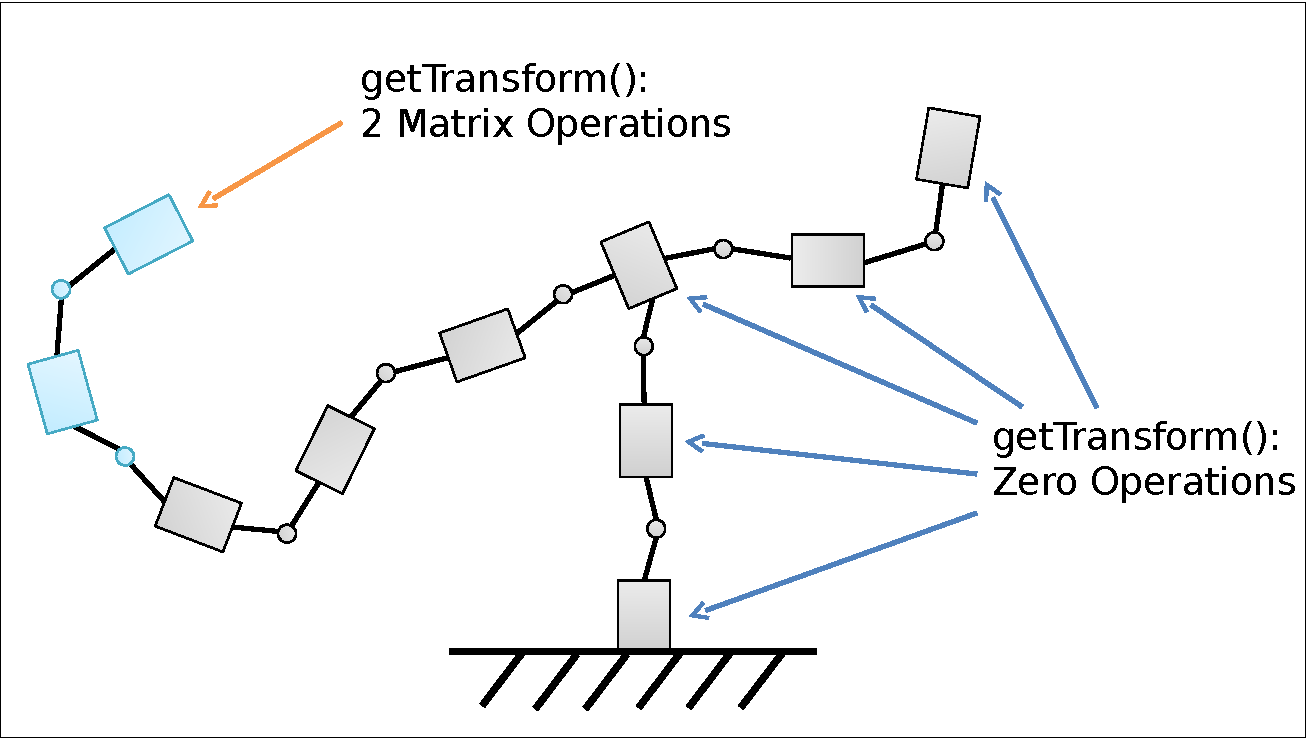
\includegraphics[width=0.44\textwidth]{fig/lazy_5.pdf}}
  \caption{Illustration of lazy evaluation for forward kinematics}
  \label{fig:lazy}
\end{figure}

In some cases, it might be undesirable to delay the computations until the time that they are requested. For example, if a real-time controller has strict scheduling requirements, there might be a specific time window which is best suited for performing heavy computations. In that case, KIDO provides a \texttt{Skeleton::computeForwardKinematics()} function which will compute all the forward kinematics within a Skeleton instead of waiting for it to be automatically updated. There are also \texttt{Skeleton::computeForwardDynamics()} and \texttt{Skeleton::computeInverseDynamics()} functions which will compute all the various dynamics parameters instead of waiting to evaluate them as needed.

\subsubsection{Exceptions: Forward and Inverse Dynamics Updating}
\label{sec:lazy_exception}
Even though forward kinematics is updated automatically, neither forward nor inverse dynamics have this quality. Individual dynamics parameters---such as the mass matrix, Coriolis forces, and articulated inertia---are updated automatically, but KIDO will \textbf{not} automatically compute the body accelerations due to the current joint torques or vice versa. This is due to the ambiguous nature of how the user might want to utilize the library: Do they want to simulate forward to see a result or compute the inverse dynamics to inform a controller? In order to compute one or the other automatically, the library would need to make an assumption about which one the user is interested in, but KIDO is meant to be suitable for both. Instead, KIDO requires the user to specifically request one or the other each time they want the results:

\begin{itemize}
  \item \textbf{\texttt{Skeleton::computeForwardDynamics()}} should be used to compute the accelerations of all the BodyNodes given the current generalized forces (or more generally, the current commands) of their joints.
  \item \textbf{\texttt{Skeleton::computeInverseDynamics()}} should be used to compute the generalized forces needed by the joints in order to achieve the current accelerations of the BodyNodes.
\end{itemize}

The results of each call will show up in the joint states of the Skeleton. The results of \texttt{computeForwardDynamics()} will show up in \texttt{Joint::getAccelerations()} and then by extension \texttt{BodyNode::getSpatialAcceleration()}, \texttt{getLinearAcceleration()}, and \texttt{getAngularAcceleration()}. The results of \texttt{computeInverseDynamics()} will show up in \texttt{Joint::getForces()} and by extension \texttt{Skeleton::getForces()}.

In both cases, the functions make use of kinematics and dynamics parameters which are cached and lazily evaluated, so making redundant calls to these functions is not prohibitively expensive, although it is still not completely free of charge.

\subsection{Extensible data structures}

There are countless applications for kinematics and dynamics software, and the developers of KIDO do not anticipate that we could possibly account for all use cases. Instead of limiting the potential applications of the library with a closed-off design, we have made the kinematics and dynamics structures extensible by introducing the concepts of \textbf{Addon}s and \textbf{Node}s.

\textbf{Addon}s and \textbf{Node}s have some practical and semantic differences, but their overarching motivation is the same: They provide a way to embed arbitrary data and functionality into kinematic and dynamic structures. For example, if you want to have a custom sensor type that can be attached to a body on your robot, you could create a custom \textbf{Node} and attach instances of your \textit{SensorNode} on whichever bodies need it.

Any concept can be encapsulated into either an \textbf{Addon} or a \textbf{Node} as long as its contents can be decomposed into a \textbf{State} structure and/or a \textbf{Properties} structure (or neither if the concept contains no information at all). To fully understand whether an Addon or a Node should be used for your purposes, the following subsections will explain the difference, but the differences can be boiled down to these:

\begin{itemize}
  \item A \textbf{BodyNode} can only contain a single instance of any particular type of \textbf{Addon}, but it can contain arbitrarily many of any particular type of \textbf{Node}.
  \item \textbf{Node}s can only be attached to \textbf{BodyNode}s, but \textbf{Addon}s can be attached to any class that inherits \textbf{AddonManager} (e.g. \textbf{Joint}, \textbf{Skeleton}, \textbf{EndEffector}).
\end{itemize}

\subsubsection{Addons}
\label{sec:addons}

There may be times where you have developed a novel algorithm that requires extra contextual information that might not be natively available in KIDO. For example, you might have computed an occupancy grid for some geometry, but KIDO does not natively support occupancy grids. Nevertheless, you want the information to be embedded in the geometric object; you want it to be saved as part of the object's \textbf{Properties}, and you want it to get copied over whenever the object is cloned.

You could achieve this by defining an \textit{OccupancyGrid} class that inherits the \textbf{Addon} class. Then you could embed an instance of an \textit{OccupancyGrid} class into the \textbf{ShapeNode} instance that holds the geometric data for which the occupancy grid was calculated:

\begin{lstlisting}
shapeNode->create<OccupancyGrid>(gridInfo);
\end{lstlisting}

You can then retrieve it with:

\begin{lstlisting}
OccupancyGrid* grid = shapeNode->get<OccupancyGrid>();
\end{lstlisting}

If the object named \texttt{shapeNode} has never created or been given an \texttt{OccupancyGrid} object, this function will return a \texttt{nullptr} by default. It is always a good idea to check whether the \textbf{Addon} pointer that gets returned is a \texttt{nullptr}, because KIDO does not throw any exceptions or assertions when you request an \textbf{Addon} that is not present in the object.

There are many native Addons in KIDO:

\begin{itemize}
  \item \textbf{Support} which is an Addon for \textbf{EndEffector}
  \item \textbf{RevoluteJoint::Addon} which contains unique properties for \textbf{RevoluteJoint}
  \item \textbf{PrismaticJoint::Addon} which contains unique properties for \textbf{PrismaticJoint}
  \item (All the other six Joint-type Addons)
  \item \todo[MXG]{Mention the Addons for ShapeFrame once they are finished}
\end{itemize}

In some cases, such as the Joint-type Addons, the Addon is crucial for the object to function correctly. In other cases, such as the \textbf{Support} class, the Addon simply provides extra features. It might seem counter-intuitive to put critical property information into an Addon if the class cannot function without it, but there is a strong motivation for this: When the \textbf{Skeleton::ExtendedProperties} is retrieved, it pulls in all the \textbf{Properties} of all the \textbf{BodyNode}s, \textbf{Node}s, and \textbf{Joint}s in the \textbf{Skeleton}, as well as the \textbf{Properties} of all the \textbf{Addon}s attached to those \textbf{BodyNode}s, \textbf{Node}s, and \textbf{Joint}s. This means that there is no special handling required in order to save all the unique property information for each different Joint-type; all their unique properties are stored in \textbf{Addon}s, and the Properties of those \textbf{Addon}s will get sucked into the \textbf{Skeleton::ExtendedProperties} automatically.

By creating your own custom Addons and attaching them to objects in Skeletons, you can extend the scope of a Skeleton's \textbf{State} and \textbf{ExtendedProperties}. The State of your Addon will be embedded into the \textbf{Skeleton::State}, and the Properties of your Addon will be embedded into the \textbf{Skeleton::ExtendedProperties}. Creating your own custom Addon involves---at a minimum---inheriting the class \textbf{kido::common::Addon} and then overriding the \textbf{Addon::cloneAddon} function. Additionally, if your Addon has a \textbf{State}, then you should also override the functions \textbf{Addon::setAddonState(const State\&)} and \textbf{Addon::getAddonState()}. Neglecting to override those functions will cause \textbf{Skeleton::State} to treat your Addon as though it has no State. Similarly, if your Addon has \textbf{Properties}, then you should override the functions \textbf{Addon::setAddonProperties(const Properties\&)} and \textbf{Addon::getAddonProperties()}. Neglecting to override these will cause \textbf{Skeleton::ExtendedProperties} to treat your Addon as though it has no Properties. Also note that the constructor of your Addon is expected to take an \textbf{AddonManager*} as its first argument; it can have any number of arbitrary argument types after that.

The most common use case of an Addon is to embed plain old data (POD) into the Properties or State of a Skeleton. To accommodate this, we offer two templated classes which take care of constructing an Addon with \textbf{State} and/or \textbf{Properties} that can live happily within a Skeleton:

\begin{itemize}
  \item \textbf{AddonWithProtectedPropertiesInSkeleton} is suitable for Addons which only has a POD \textbf{Properties} and no \textbf{State}.
  \item \textbf{AddonWithProtectedStateAndPropertiesInSkeleton} is suitable for Addons which have both a POD \textbf{State} and a POD \textbf{Properties}.
\end{itemize}

The template arguments of these classes work as follows:

\begin{itemize}
  \item The class type that inherits this class. These are CRTP classes.
  \item (Only for AddonWithProtectedStateAndPropertiesInSkeleton) The POD \textbf{State} type
  \item The POD \textbf{Properties} type
  \item The type of AddonManager that this class is intended for. Pass in \texttt{AddonManager} if the type of AddonManager is irrelevant.
  \item (Only for AddonWithProtectedStateAndPropertiesInSkeleton) The function that should be called whenever the State of the Addon is updated.
  \item The function that should be called whenever the Properties of the Addon are updated
\end{itemize}

The update functions that are used for the final template argument(s) must accept a single argument, which will be a pointer to the full Addon class. CRTP (Curiously Recurring Template Pattern) is used to make this possible.

The \textbf{State} and \textbf{Properties} are protected for this type of Addon to ensure that all changes to the \textbf{Properties} are registered by the \textbf{Skeleton}. Otherwise, \textbf{Skeleton}s would not be able to correctly keep track of their ``version'' number \todo[MXG]{We should probably have a section about Skeleton version and cite it here}. This can be inconvenient if the POD \textbf{State} or \textbf{Properties} structures have many fields that need to be accessed or changed, because then accessor and mutator functions are needed for each one. This can entail a troublesome amount of typing, and worse yet: When writing mutator functions, you must be sure to call the correct update functions, and increment the Skeleton's version number if a property is being changed.

To avoid the hassle and dangers of writing many accessor and mutator functions, KIDO provides a few macros which can take of this:

\paragraph{KIDO\_DYNAMICS\_SET\_GET\_ADDON\_PROPERTY} will create a setter and getter function for a variable in the Properties POD. The first argument for this macro is the variable type, and the second argument is the variable name. There is also:
\begin{itemize}
  \item \textbf{KIDO\_DYNAMICS\_SET\_ADDON\_PROPERTY} which will only create the set
  \item \textbf{KIDO\_DYNAMICS\_GET\_ADDON\_PROPERTY} which will only create the get
\end{itemize} 

\paragraph{KIDO\_DYNAMICS\_SET\_GET\_ADDON\_PROPERTY\_ARRAY} can be used to access and mutate the individual components of an array or vector field within the POD \textbf{Properties} structure. For variable names whose plural form is ``irregular'' (i.e. is not the same as adding `s' to the end), there is also 

\begin{itemize}
  \item \textbf{KIDO\_DYNAMICS\_IRREGULAR\_SET\_GET\_ADDON\_PROPERTY\_ARRAY} which allows you to specify the singular and plural forms of the name.
\end{itemize}

There are more macros, similar to these, which address a variety of use cases. Although C-macros can be strange and clumsy, they can save a significant amount of typing and prevent errors that may result from forgetfulness.

\subsubsection{Nodes}
\label{sec:nodes}
\red{Grey}
\subsection{History recorder}
\todo[MXG]{It doesn't look like we'll have this in time for the next major release, although it will probably be available for the next minor release. Will it be possible to update this tech report as we add features and make changes?}
\subsection{Optimization interface}
\label{sec:optimizer}
\red{Grey}
\subsection{Extensible GUI}
\red{JS}

%\section{Lesson 0: Simulate a passive multi-pendulum}

This is a warmup lesson that demonstrates how to set up a simulation program in DART. The example we will use throughout this tutorial is a pendulum with five rigid bodies swinging under gravity. DART allows the user to build various articulated rigid/soft body systems from scratch. It also loads models in URDF, SDF, and SKEL formats as demonstrated in the later tutorials.

In DART, an articulated dynamics model is represented by a \textbf{Skeleton}. In the main function, we first create an empty skeleton named \emph{pendulum}.

\begin{lstlisting}
SkeletonPtr pendulum = Skeleton::create("pendulum");
\end{lstlisting}

A Skeleton is a structure that consists of \textbf{BodyNode}s (bodies) which are connected by \textbf{ Joint}s. Every Joint has a child BodyNode, and every BodyNode has a parent Joint. Even the root BodyNode has a Joint that attaches it to the \textbf{World}. In the function makeRootBody, we create a pair of a \textbf{BallJoint} and a BodyNode, and attach this pair to the currently empty pendulum skeleton.

\begin{lstlisting}
BodyNodePtr bn = pendulum->createJointAndBodyNodePair<BallJoint>(nullptr, properties, BodyNode::Properties(name)).second;
\end{lstlisting}

Note that the first parameters is a nullptr, which indicates that this new BodyNode is the root of the pendulum. If we wish to append the new BodyNode to an existing BodyNode in the pendulum, we can do so by passing the pointer of the existing BodyNode as the first parameter. In fact, this is how we add more BodyNodes to the pendulum in the function addBody:

\begin{lstlisting}
BodyNodePtr bn = pendulum->createJointAndBodyNodePair<RevoluteJoint>(parent, properties, BodyNode::Properties(name)).second;
\end{lstlisting}

The simplest way to set up a simulation program in DART is to use SimWindow class. A SimWindow owns an instance of World and simulates all the Skeletons in the World. In this example, we create a World with the pendulum skeleton in it, and assign the World to an instance of \textbf{MyWindow}, a subclass derived from \textbf{SimWindow}.

\begin{lstlisting}
WorldPtr world(new World);
world->addSkeleton(pendulum);
MyWindow window(world);
\end{lstlisting}

Every single time step, the MyWindow::timeStepping function will be called and the state of the World will be simulated. The user can override the default timeStepping function to customize the simulation routine. For example, one can incorporate sensors, actuators, or user interaction in the forward simulation.

\section{Lesson 1: Change shapes and applying forces}

We have a pendulum with five bodies, and we want to be able to apply forces to them during simulation. Additionally, we want to visualize these forces so we can more easily interpret what is happening in the simulation. For this reason, we'll discuss visualizing and forces at the same time.

\subsection{Lesson 1a: Reset everything to default appearance}

At each step, we'll want to make sure that everything starts out with its default appearance. The default is for everything to be blue and there not to be any arrow attached to any body. Find the function named timeStepping in the \textbf{MyWindow} class. The top of this function is where we will want to reset everything to the default appearance.

Each BodyNode contains visualization \textbf{Shape}s that will be rendered during simulation. In our case, each BodyNode has two shapes: One shape to visualize the parent joint and one shape to visualize the body. The default appearance for everything is to be colored blue, so we'll want to iterate through these two Shapes in each BodyNode, setting their colors to blue.

\begin{lstlisting}
for(size_t i = 0; i < mPendulum->getNumBodyNodes(); ++i)
{
  BodyNode* bn = mPendulum->getBodyNode(i);
  for(size_t j = 0; j < 2; ++j)
  {
    const ShapePtr& shape = bn->getVisualizationShape(j);

    shape->setColor(dart::Color::Blue());
  }
  // TODO: Remove any arrows
}
\end{lstlisting}

Additionally, there is the possibility that some BodyNodes will have an arrow shape attached if the user had been applying an external body force to it. By default, this arrow should not be attached, so in the outer for-loop, we should check for arrows and remove them:

\begin{lstlisting}
if(bn->getNumVisualizationShapes() == 3)
{
  bn->removeVisualizationShape(mArrow);
}
\end{lstlisting}



\pagebreak
\thispagestyle{empty}
\pagestyle{empty}
\bibliographystyle{unsrt}
\bibliography{refs.bib}

\end{document}
